\documentclass[letterpaper,12pt]{article}
\usepackage[utf8]{inputenc}
\usepackage{amsmath}
\usepackage{amsfonts}
\usepackage{amssymb}
\usepackage{enumerate}
\usepackage[margin=0.75 in]{geometry}
\usepackage{graphicx}
\usepackage{hyperref}

\newcommand{\aaa}{\mathbf{a}}
\newcommand{\bbb}{\mathbf{b}}
\newcommand{\abs}[1]{\lvert #1\rvert}
\newcommand{\len}[1]{\lVert #1\rVert}
\newcommand{\dotp}{\boldsymbol{\cdot}}
\renewcommand{\r}{\mathbf{r}}
\newcommand{\x}{\mathbf{x}}
\newcommand{\R}{\mathbb{R}}
\newcommand{\di}{\displaystyle}
%opening
\title{So you want to do a limit proof in several variables\\Math 2580, Spring 2016}
\author{Sean Fitzpatrick}

\begin{document}

\maketitle

As discussed in class, once we move from one to two or more variables, limits become quite a bit trickier due to the fact that there are infinitely many ways to approach a given point. In fact, the situation is worse than the fact that there are infinitely many directions in two or more dimensions (this infinity being a relatively small one, so to speak\footnote{There are, by the way, different ``sizes'' of infinity. This issue is not one for this course, but if you're curious, you may want to see what Google or Wikipedia can tell you about the work of Georg Cantor. This is something that is usually discussed in Math 2000.}). Consider the limit $\di \lim_{(x,y)\to (0,0)}\frac{x^2y}{x^4+y^2}$: the limit is zero if we approach along either the $x$-axis or the $y$-axis, and indeed, we could consider a more general straight line through the origin of the form $y=mx$. Along such a line, the limit becomes
\[
 \lim_{(x,y)\to (0,0)}\frac{x^2y}{x^4+y^2} = \lim_{x\to 0} \frac{mx^3}{x^4+m^2x^2} = \lim_{x\to 0} \frac{mx}{m^2+1} = 0.
\]
At this point we should be pretty confident that the limit is zero - after all, we've considered every possible direction along which we could approach the origin, right? Unfortunately, this is not enough: we need to verify that the limit is zero for every possible {\em path}, and this is simply an impossible task! However, in this case we {\em can} show that the limit {\em doesn't} exist by staring at the function for a bit, noticing that $x$ appears top and bottom with twice the power of $y$, and then asking what happens if $y=x^2$. When this is the case, we find
\[
  \lim_{(x,y)\to (0,0)}\frac{x^2y}{x^4+y^2} = \lim_{x\to 0}\frac{x^4}{x^4+x^4} = \frac{1}{2}\neq 0,
\]
and we're forced to conclude that the limit does not exist. If you're wondering what such a surface might look like, here's a rendering using K3dSurf. (It's not perfect, but you can see the parabolic arcs along which the function is constant.)
\begin{center}
 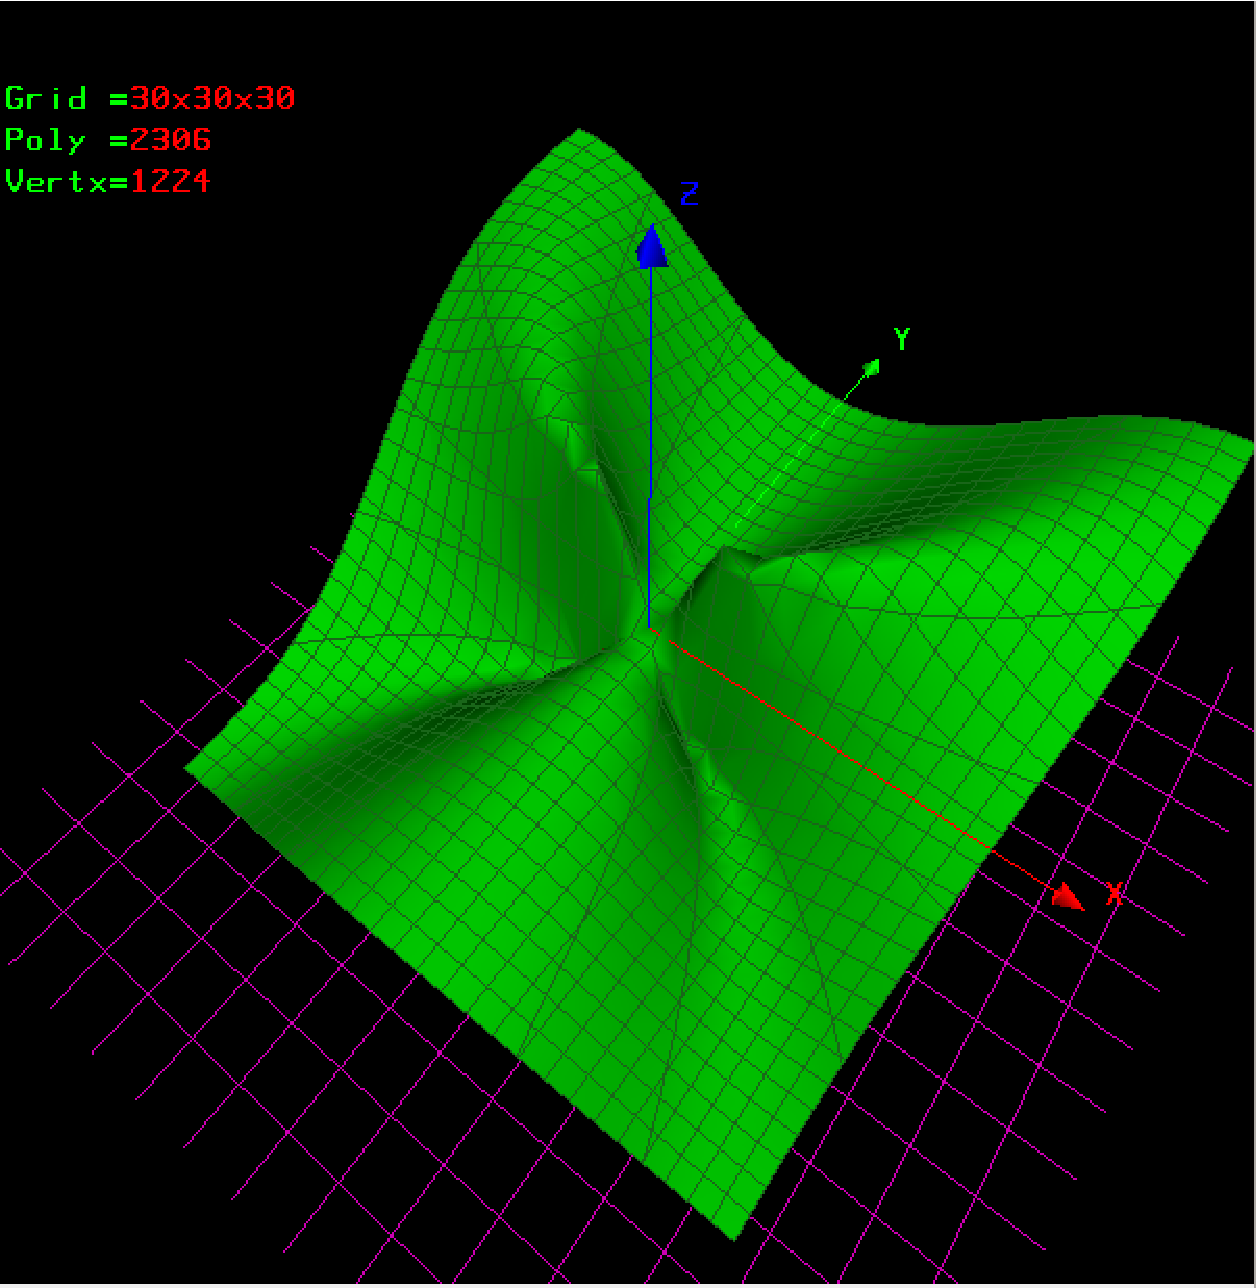
\includegraphics[width=4in]{parabolic_limit.pdf}
\end{center}
The upshot of all this is that for functions of several variables, we're forced to rely on the precise definition of a limit if we want to prove anything. Let's recall the definition: we say that the limit of $f(x,y)$ at a point $(a,b)$ is $L$, and write $\di \lim{(x,y)\to(a,b)}f(x,y)=L$, if for every $\epsilon>0$ there exists a $\delta>0$ such that 
\[
 \text{If } 0<\sqrt{(x-a)^2+(y-b)^2}<\delta, \text{ then } \abs{f(x,y)-L}<\epsilon.
\]
For this to make sense, the point $(a,b)$ needs to be such that every $\epsilon$ neighbourhood $N_\epsilon(a,b)$ of $(a,b)$ contains points in the domain of $f$, which means that either $(a,b)$ is itself in the domain of $f$, or it's on the boundary of of the domain. (The definitions of neighbourhoods and boundary points were given in Friday's lecture.) We can make a similar definition for functions of three or more variables. Notationally, it's convenient to identify points with their position vectors, and write
\[
 \lim_{\x\to\aaa}f(\x)=L \,\Leftrightarrow\, \text{ For all } \epsilon>0 \text{ there exists } \delta>0 \text{ such that } 0<\len{\x-\aaa}<\delta \Rightarrow \abs{f(\x)-L}<\epsilon
\]
In terms of neighbourhoods, we could also write $\x\in N_\delta(\aaa)\cap D$ implies $f(\x)\in N_\epsilon(L)$, where $D$ denotes the domain of $f$. (Since $\aaa$ might be a boundary point of $D$, we take the intersection with $D$ to ensure that $f(\x)$ is defined.)

\medskip

For example, suppose we want to prove that $\di \lim_{(x,y)\to (1,2)}(2x+y)=4$. We start by supposing that someone has specified the number $\epsilon$, telling us how far away from 4 we need to make $f(x,y)=2x+y$, but we don't say specifically what the value of $\epsilon$ is, because we want our argument to work no matter what value is chosen. We then need to choose a value for $\delta$, which usually depends on $\epsilon$ and the function. What should $\delta$ be? Well, we need to do a bit of work to find out. We're trying to show that we can make $\abs{2x+y-4}$ as small as we want. The strategy for this might seem strange at first: we start by replacing the thing we want to make small by things that are {\em bigger}. The reason for this is simple, however: if we can find something bigger than $\abs{2x+y-4}$, and show that we can make {\em that} as small as we want, then it follows that $\abs{2x+y-4}$ must be even smaller. (Think of this as being like a squeeze theorem argument.) So, we play around with $\abs{2x+y-4}$ a bit, keeping in mind that we're considering values of $x$ close to 1, and $y$ close to 2. We have
\[
 \abs{2x+y-4} = \abs{2x-2+y-2} = \abs{2(x-1)+(y-2)} \leq 2\abs{x-1}+\abs{y-2}.
\]
In the last step we used the triangle inequality, and now we have everything in terms of $\abs{x-1}$ and $\abs{y-2}$, which is exactly what we want: notice that
\[
 \abs{x-1} = \sqrt{(x-1)^2}\leq \sqrt{(x-1)^2+(y-2)^2},
\]
and similarly $\abs{y-2}\leq \sqrt{(x-1)^2+(y-2)^2}$. This means that if $\sqrt{(x-1)^2+(y-2)^2}<\delta$, we have $\abs{x-1}<\delta$ and $\abs{y-2}<\delta$ as well, and then our argument above tells us that $\abs{2x+y-4} \leq 2\abs{x-1}+\abs{y-2}<2\delta+\delta=3\delta$. Thus, if we want to make $\abs{2x+y-4}<\epsilon$, all we have to do is choose $\delta$ so that $3\delta\leq \epsilon$. With this groundwork in place, we can write our proof, which looks something like this:

\medskip

Let $\epsilon>0$ be given, and choose $\delta = \epsilon/3$. If we suppose that $0<\sqrt{(x-1)^2+(y-2)^2}<\delta$, then in particular $\abs{x-1}<\delta$ and $\abs{y-2}<\delta$, and therefore
\[
 \abs{2x+y-4} = \abs{2(x-1)+(y-2)} \leq 2\abs{x-1}+\abs{y-2}<2\delta+\delta = 3\delta = \epsilon.
\]
Thus, it follows from the definition of the limit that $\di \lim_{(x,y)\to (1,2)}(2x+y)=4$.

\medskip

As mentioned in class, all of the usual limit laws continue to hold for several variables. In particular, let $f,g:D\subseteq\R^n\to \R$ be given functions (with $n=2$ or 3), and let $c\in\R$ be a constant. If $\di \lim_{\x\to\aaa}f(\x) = L$ and $\di \lim_{\x\to\aaa}g(\x)=M$, then
\begin{enumerate}
 \item $\lim_{\x\to\aaa}(f(\x)+g(\x)) = L+M$
 \item $\lim_{\x\to\aaa}(cf(\x)) = cL$
 \item $\lim_{\x\to\aaa}(f(\x)g(\x)) = LM$
 \item $\lim_{\x\to\aaa}\dfrac{f(\x)}{g(\x)} = \dfrac{L}{M}$, provided $M\neq 0$.
\end{enumerate}
The proof of each of these is the same as it is in one variable. For example, the proof of (1) is as follows:

\medskip

Let $\epsilon>0$ be given. Since $\di \lim_{\x\to\aaa}f(\x) = L$ and $\di \lim_{\x\to\aaa}g(\x)=M$, there exists a $\delta_1>0$ such that $0<\len{\x-\aaa}<\delta_1$ implies that $\abs{f(\x)-L}<\epsilon/2$, and a $\delta_2>0$ such that $0<\len{\x-\aaa}<\delta_2$ implies that $\abs{g(\x)-M}<\epsilon/2$. Choose $\delta$ to be the minimum of $\delta_1$ and $\delta_2$, and suppose that $0<\len{\x-\aaa}<\delta$. Then
\[
 \abs{(f(\x)+g(\x))-(L+M)} = \abs{(f(\x)-L)+(g(\x)-M)}\leq \abs{f(\x)-L}+\abs{g(\x)-M}<\epsilon/2+\epsilon/2=\epsilon.
\]
The proof for the product law is a bit trickier. For a proof of the one-variable case, see here: \href{http://planetmath.org/ProofOfLimitRuleOfProduct.html}{http://planetmath.org/ProofOfLimitRuleOfProduct.html}. To make it into a two-variable proof, you only need to replace the $\abs{x-a}$ terms with $\len{\x-\aaa}$.

\bigskip

Once limits are defined properly, continuity can be defined in the same way as usual: we say that a function $f:D\subseteq\R^n$ is {\em continuous} at a point $\aaa\in D$ if $\di \lim_{\x\to \aaa}f(\x) = f(\aaa)$. It's easy to check that the functions $f(x,y)=x$ and $g(x,y)=y$ are continuous everywhere, and then the limit laws allow us to conclude that any polynomial or rational function in several variables is continuous on its domain. In addition (as you'll show on your assignment) the composition of continuous functions is continuous, and this immediately lets us conclude that, for example, a function such as $f(x,y,z) = x\sin(yz)$ is continuous on all of $\R^3$.

\bigskip

Let's look at one more example of an $\epsilon-\delta$ proof in two variables. There are lots of additional examples available online if you'd like to see more. Let's use the definition of the limit to show that
\[
 \lim_{(x,y)\to (1,0)}\frac{x+y+1}{x+2y} = 2.
\]
(This result also follows from the limit laws.) We start with the object we want to make small. We have
\[
 \left|\frac{x+y+1}{x+2y}-2\right| = \left|\frac{1-x-3y}{x+2y}\right|\leq \left|\frac{x-1}{x+2y}\right|+3\left|\frac{y}{x+2y}\right|.
\]
Now, we know that we can make $\abs{x-1}$ and $\abs{y}$ as small as we want, but we also have to make sure that the denominator $x+2y$ doesn't get too small, or it might make the overall fraction really big. The best way to do this is to take a ``test value'' for $\delta$. If $\delta=1$, then $\abs{x-1}<1$ gives $0<x<2$, and $\abs{y}<1$ gives $-1<y<1$. But now we see that we have a problem with this test value: there is nothing stopping us from having $x+2y$ arbitrarily close to zero! Let's try $\delta = 1/4$ instead. In that case, $\abs{x-1}<1/4$ gives $3/4<x<5/4$, and $\abs{y}<1/4$ gives $-1/4<y<1/4$. This tells us that $x+2y$ can't get any smaller than $3/4+2(-1/4) = 1/4$. We're now ready to give our proof.

\medskip

Let $\epsilon>0$ be given, and take $\delta$ to be the minimum of  $\epsilon/16$  and $1/4$. Suppose that $0<\sqrt{x-1)^2+y^2}<\delta$. Then in particular $\abs{x-1}<1/4$ and $\abs{y}<$ from which it follows that $2x+y>1/4$, and thus $\dfrac{1}{2x+y}<4$. We then have
\[
 \left|\frac{x+y+1}{x+2y}-2\right| = \left|\frac{1-x-3y}{x+2y}\right|\leq \frac{\abs{x-1}}{\abs{x+2y}}+3\frac{\abs{y}}{\abs{x+2y}}<4\abs{x-1}+12\abs{y}<16\delta<\epsilon.
\]

\bigskip

We end with a remark about using polar coordinates for limits in two variables. In some cases a limit that would otherwise need an $\epsilon-\delta$ proof can be handled using polar coordinates. (This method is mentioned in Stewart's textbook but isn't completely justified.) Suppose we want to prove that $\di\lim_{(x,y)\to (a,b)}f(x,y)=L$. If we let $x=a+r\cos\theta$ and $y=b+r\sin\theta$, then 
\[
\sqrt{(x-a)^2+(y-b)^2} = \sqrt{r^2\cos^2\theta+r^2\sin^2\theta} = \abs{r},
\]
so that $0<\sqrt{(x-a)^2+(y-b)^2}<\delta$ if and only if $0<\abs{r}<\delta$. It follows that
\[
\lim_{(x,y)\to (a,b)}f(x,y) = \lim_{r\to 0}f(a+r\cos\theta,b+r\sin\theta),
\]
so that we need only consider the single variable limit in terms of $r$. (Note however that in order for this limit to exist, it cannot depend on $\theta$.) For example, we have
\[
\lim_{(x,y)\to (0,0)}\frac{x^4+y^2}{x^2+y^2} = \lim_{r\to 0}\frac{r^4\cos^4\theta+r^2\sin^2\theta}{r^2} = \lim_{r\to 0}(r^2\cos^2\theta+\sin^2\theta)=\sin^2\theta.
\]
Since the end result still depends on $\theta$, the limit must not exist. However, if we replace the $y^2$ in the denominator by $y^3$, then we see that the limit will be zero.

\end{document}
